\documentclass{dit}

\usepackage{amsmath}
\usepackage{hyperref}
\pdfstringdefDisableCommands{\def\_{_}}
\usepackage{tikz}
% \usepackage{pgfplots}

% allow embedding files in the PDF so viewers can open/save them
\usepackage{attachfile2}

% CSV import for tables
\usepackage{csvsimple}
\usepackage{longtable}
% ensure floats appear before section text when desired
\usepackage{placeins}
% code/listing support for run commands
\usepackage{listings}
\lstset{basicstyle=\ttfamily\small,breaklines=true,columns=fullflexible}

% Macro to show how to run binaries in a consistent way
\newcommand{\runcmd}[1]{\vspace{6pt}\noindent\textbf{Run: }\lstinline!#1!\par}

\usepackage[english,greek]{babel}
% helper to typeset short English fragments when main language is Greek
\newcommand{\en}[1]{\foreignlanguage{english}{#1}}

\newcommand*{\name}{Ευάγγελος Τραϊκόγλου}
\newcommand*{\id}{1115202200189}
\newcommand*{\course}{Παράλληλα Συστήματα}
\newcommand*{\assignment}{Εργασία \en{Simd}}

\begin{document}

\maketitle

% \tableofcontents
\begin{itemize}
    \item \en{cpu}: \en{i7-8700}
    \item \en{cores}: \en{12 logical, 6 physical}
    \item \en{os, kernel}: \en{Ubuntu 24.04.3 LTS, 6.8.0-94-generic}
    \item \en{comp version}: \en{gcc 13.3.0}
\end{itemize}


\section*{\en{Polynomial Multiplication}}
Η άσκηση επικεντρώνεται στον πολλαπλασιασμό πολυωνύμων βαθμού \en{n}.
Ο σειριακός αλγόριθμος ακολουθεί την απλή υλοποίηση $\mathcal{O}(n^2)$ χρόνου.
Για την παράλληλη εκδοχή υπάρχουν 2 υλοποιήσεις γιατί παρατηρήθηκε ότι με τα \en{optimize flags off}
κάθε \en{update} που γινόταν σε 1 \en{register} είχε ως αποτέλεσμα την άμεση καταγραφή και στο \en{stack}
παρόλο που δεν χρειαζόταν αφού θα χρησιμοποιούνταν αμέσως μετά. Αυτό ήταν το κύριο \en{bottleneck}. Απ' ότι
διάβασα είναι για λόγους \en{debugging}. Οπότε υπάρχει και 2 υλοποίηση (\en{simd\_mul\_O1}) που χρησιμοποιεί το
\en{O1 flag} και η διαφορά στο χρόνο είναι σημαντική: $\backsim$  \en{2.3sec, 100k degree input}.
Στην \en{simd\_mul\_O1}, χρησιμοποιούνται \en{simd} εντολές \en{256bit/8 elements (load,store,add,multiply)}. 
Ακόμη ο βρόχος ξετυλίγεται (4 επαναλήψεις, \en{saves 2.2sec on 100k degree input}).
\\\\
\underline{Σημείωση}: 
Το \en{base} για τα \en{optimizations} που εξηγούνται παρακάτω είναι η \en{simd\_mul\_O1} χωρίς το \en{directive}
για \en{optimize}.
\\
Στην \en{simd\_mul} έγιναν κάποιες βελτιστοποιήσεις με το χέρι. Όπως ειπώθηκε το βασικό πρόβλημα είναι τα
αχρείαστα \en{store} στο \en{stack}. Για αυτό το λόγο προστέθηκε το \en{directive ACCUMULATE\_8} που εμφωλευμένα
καλεί όλα τα \en{calls} που πρέπει να γίνουν για την 8άδα στοιχείων (\en{load,mult,add,store}). Αυτό εξαλείφει
μερικά \en{stack writes} και ρίχνει τον χρόνο ($\backsim$ 0.6\en{sec} για \en{100k degree pol}). Ακόμα το \en{pointer
arithmetic} για να βρεθεί η επόμενη θέση έναντι του απλού \en{access, eg: a[i+j]} ρίχνει τον χρόνο κάτα \en{1.3sec, 100k pol\_deg}.
Τέλος, το \en{prefetch} του επόμενου \en{cache line} ρίχνει το χρόνο κατά: \en{ $\backsim$ 0.2sec 100k, $\backsim$ 1sec 200k}.
\\
\en{\runcmd{./polynomial_mult -n <degree> }}

\underline{Σημείωση}: 
Όλα τα πειράματα υπάρχουν στο \en{csv} αρχείο: \en{simd\_bench\_results.csv}.

\begin{figure}[htbp]
    \centering
    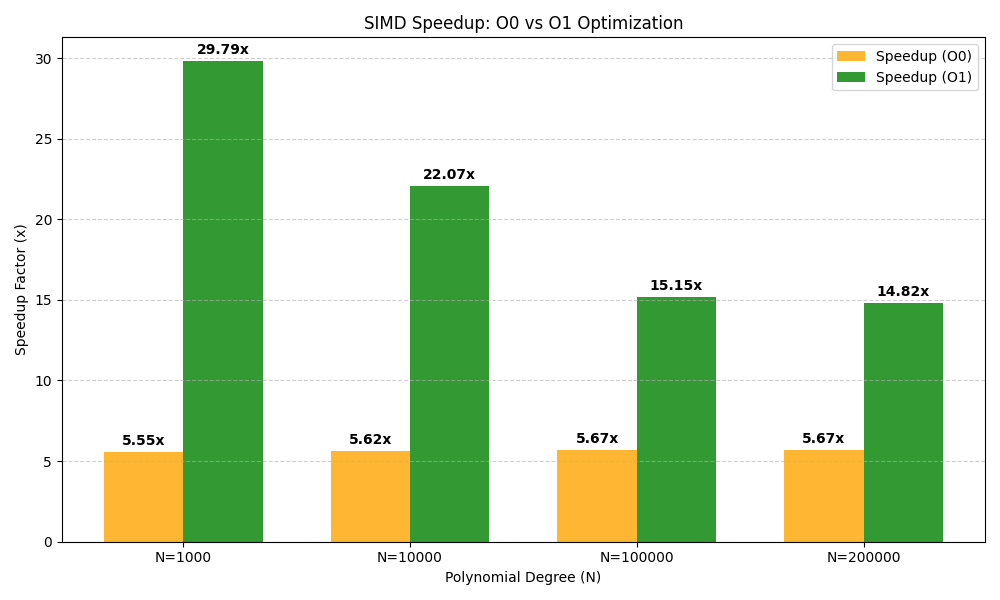
\includegraphics[width=0.8\linewidth]{graphs/speedup.png}
\end{figure}


\begin{figure}[htbp]
    \centering
    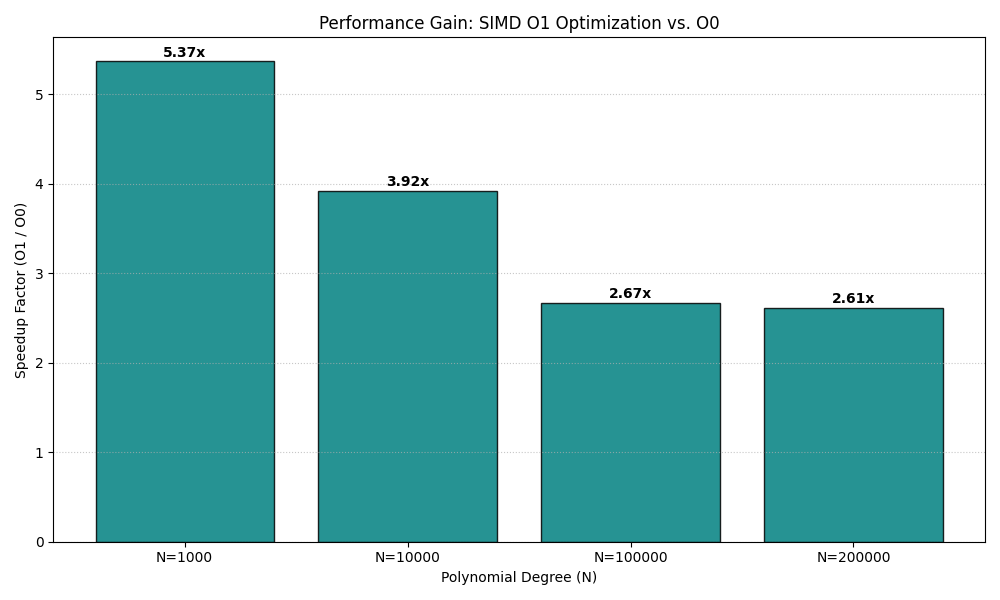
\includegraphics[width=0.8\linewidth]{graphs/speedup_O1_vs_O0.png}
\end{figure}


\FloatBarrier
\underline{Συμπεράσματα}:
Η επιτάχυνση που παρατηρείται είναι σταθερή ($\backsim$ 5.6) για όλα τα μεγέθη πολυωνύμων 
αφού χρησιμοποιείται το ίδιο μοτίβο γενικά της επεξεργασίας 8 στοιχείων τη φορά μέσω \en{vector registers}. 
Το βασικό \en{bottleneck} στη περίπτωση του \en{simd\_mul} είναι το \en{memory traffic} λόγω των αχρείαστων \en{stack writes} που
αν και μειώθηκε λόγω των βελτιστοποιήσεων, δεν εξαφανίστηκε πλήρως. Προφανώς στη περίπτωση Ο1 και άλλες βελτιστοποιήσεις
μπορεί να βοηθάνε συμπληρωματικά (πχ καλύτερο \en{scheduling} εντολών) για αυτό και παρατηρείται μεγάλη διαφορά μεταξύ
των 2 υλοποιήσεων (κυρίως στα μικρά μεγέθη), ενώ σταθεροποιείται περίπου στο $\backsim$ 2.5 η επιτάχυνση Ο1 έναντι του Ο0
στα μεγαλύτερα. 
\FloatBarrier



\end{document}